%!TeX spellcheck = en_GB
% ****** Start of file templateForReport.tex ******

% TeX'ing this file requires that you have all prerequisites
% for REVTeX 4.1 installed
%
% See the REVTeX 4 README file
% It also requires running BibTeX. The commands are as follows:
%
%  1)  latex templateForReport.tex
%  2)  bibtex templateForReport
%  3)  latex templateForReport.tex
%  4)  latex templateForReport.tex
%
\documentclass[%
 reprint,
%superscriptaddress,
%groupedaddress,
%unsortedaddress,
%runinaddress,
%frontmatterverbose,
%preprint,
%showpacs,preprintnumbers,
%nofootinbib,
%nobibnotes,
%bibnotes,
 amsmath,amssymb,
 aps,
%pra,
%prb,
%rmp,
%prstab,
%prstper,
%floatfix,
]{revtex4-1}

\usepackage{graphicx}% Include figure files
\usepackage{dcolumn}% Align table columns on decimal point
\usepackage{bm}% bold math
%\usepackage{hyperref}% add hypertext capabilities
%\usepackage[mathlines]{lineno}% Enable numbering of text and display math
%\linenumbers\relax % Commence numbering lines

%\usepackage[showframe,%Uncomment any one of the following lines to test
%%scale=0.7, marginratio={1:1, 2:3}, ignoreall,% default settings
%%text={7in,10in},centering,
%%margin=1.5in,
%%total={6.5in,8.75in}, top=1.2in, left=0.9in, includefoot,
%%height=10in,a5paper,hmargin={3cm,0.8in},
%]{geometry}

\usepackage{dsfont} % mathds for unity matrix

\usepackage{xcolor}
\usepackage{tikz}%Bilder
\usepackage{pgfpages}
\usetikzlibrary{positioning, arrows}
\usepackage{smartdiagram}%Kreisdiagramm/Flussdiagramm

\DeclareMathOperator{\Tr}{Tr}
\renewcommand{\Re}{\operatorname{Re}}

\begin{document}
	\tikzstyle{arrow} = [very thick, ->, >=stealth]

\title{Yang-Mills on the Lattice}% Force line breaks with \\
%\thanks{A footnote to the article title}%

\author{Nico Dichter}
\author{Christiane Gro\ss{}}


\date{March 2021}% It is always \today, today,
             %  but any date may be explicitly specified

\begin{abstract}
	We measure the confinement that arises when simulating a Lattice with the Yang-Mills action, by approximating the lattice links with SU(2) matrices
%  An article usually includes an abstract, a concise summary of the work
%  covered at length in the main body of the article.
%  \begin{description}
%  \item[Usage]
%    Secondary publications and information retrieval purposes.
%  \item[Structure]
%    You may use the \texttt{description} environment to structure your abstract;
%    use the optional argument of the \verb+\item+ command to give the category of each item.
%  \end{description}
\end{abstract}
\maketitle

%\tableofcontents

\section{Introduction}

%We want to calculate the potential between two infinitely heavy quarks. To do this, we first simulate an empty lattice and then use the fact that static quarks do not vary their location when the time is varied.

\section{Theoretical basis}

Most of the theoretical basis given here is adapted from \citet{lepagelqcd}. We want to discretize three spatial and one temporal dimension, so we need a four-dimensional lattice. The distance between any adjacent lattice points is $a$, and any point is characterized by four coordinates, $x=(x,y,z,t)$. The links between the lattices are characterized by an additional direction $\mu$, and we only consider the forward facing links $U_\mu(x)$ going from $x$ to $x+a\mu$. All links are represented as $SU(N)$-matrices, we simulate $N=2$ and $N=3$.backward-facing links from $x+a\mu$ to $x$ are represented by $U_\mu^\dagger(x)$.

The simplest loop that can be formed with the links of the lattice is the plaquette \[P_{\mu\nu}(x)=\frac{1}{N}\Re\Tr\left(U_\mu(x)U_\nu(x+a\mu)U_\mu^\dagger(x+a\nu)U^\dagger_\nu(x)\right)\] a simple square. The discretized action is defined as being proportional to the ordered sum over all plaquettes, \[S=\frac{2N}{g^2}\sum_{x}\sum_{\mu>\nu}\left(1-P_{\mu\nu}(x)\right)+\mathcal{O}(a^2)\]
and $\beta=\frac{2N}{g^2}$ is the coupling strength. 

%Some citation \citet{gsldoc_complex}

%Most of the theoretical basis given here is adapted from \citet{lepagelqcd}. We simulate a lattice with one temporal and three spatial dimensions, with the distande $a$ between neighbouring points. The nearest neighbours in this lattice are linked, with the links characterized by SU(2) or SU(3) matrices $U_\mu(x)$, where $\mu=0\dots3$ is the direction of the link. Backwards links are defined as the hermitian adjoint of the forward-facing link. The plaquette is the smallest possible square on the lattice and is defined as $P_{\mu\nu}(x)=\frac{1}{N}\Re\Tr\left(U_\mu(x)U_\nu(x+a\mu)U_\mu^\dagger(x+a\nu)U^\dagger_\nu(x)\right)$, where $N$ describes the dimension of the unitary matrices used to simulate the links. Building on this, we define the action to be $S=\frac{2N}{g^2}\sum_{x}\sum_{\mu>\nu}\left(1-P_{\mu\nu}(x)\right)$.
%
%Definition wilson-loop: maybe draw loop? How?
%

%\[W(x, k_\mu a, l_\nu a)=U_\mu(x)\cdots U_\mu(x+(k-1)a\mu)U_\nu(x+ka\mu)\cdots U_\nu(x+ka\mu+(l-1)a\nu)U_mu^dagger\]

A general loop around a closed contour $\mathcal{C}$ is also called Wilson loop $W(\mathcal{C})$. Regarding the more complicated loops possible, we are interested in $W(R\times T)$ that go a distance $R$ in the spatial directions and a distance $T$ in the temporal direction. Their expectation values can be calculated as 

\begin{tikzpicture}[y=0.5cm, x=0.5cm,
roundnode/.style={circle, draw=white, thick, minimum size=1pt},
]
\node[roundnode]at(-4.0, 1)(equation){$W(R\times T)=\frac{1}{N}\Re\Tr$};
\node[roundnode]at(2.5, -0.8)(R){R};
\draw[arrow] (2,-0.8)--(0,-0.8);
\draw[arrow] (3,-0.8)--(5,-0.8);
\node[roundnode]at(5.8, 1)(T){T};
\draw[arrow] (5.8, 1.5)--(5.8,2);
\draw[arrow] (5.8, 0.5)--(5.8,0);
\filldraw[black] (0,0) circle (2pt);
\draw[arrow] (0,0)--(1,0);
\filldraw[black] (1,0) circle (2pt);
\draw[arrow] (1,0)--(2,0);
\filldraw[black] (2,0) circle (2pt);
\draw[arrow] (2,0)--(3,0);
\filldraw[black] (3,0) circle (2pt);
\draw[arrow] (3,0)--(4,0);
\filldraw[black] (4,0) circle (2pt);
\draw[arrow] (4,0)--(5,0);
\filldraw[black] (5,0) circle (2pt);
\draw[arrow] (5,0)--(5,1);
\filldraw[black] (5,1) circle (2pt);
\draw[arrow] (5,1)--(5,2);
\filldraw[black] (5,2) circle (2pt);
\draw[arrow] (5,2)--(4,2);
\filldraw[black] (4,2) circle (2pt);
\draw[arrow] (4,2)--(3,2);
\filldraw[black] (3,2) circle (2pt);
\draw[arrow] (3,2)--(2,2);
\filldraw[black] (2,2) circle (2pt);
\draw[arrow] (2,2)--(1,2);
\filldraw[black] (1,2) circle (2pt);
\draw[arrow] (1,2)--(0,2);
\filldraw[black] (0,2) circle (2pt);
\draw[arrow] (0,2)--(0,1);
\filldraw[black] (0,1) circle (2pt);
\draw[arrow] (0,1)--(0,0);
\filldraw[black] (0,0) circle (2pt);
\end{tikzpicture}

We want to determine the potential between two infinitely heavy, static quarks. We know
$\langle W(R\times T)\rangle\sim \mathrm{e}^{aV(R)T}$%\Leftrightarrow \frac{W(r,t+a)}{W(r,t)}\sim aV(r)$
and thus calculating the values of the Wilson-loops for different $T$ and $R$ allows us to extract the potential. 

The potential is expected to have the form $V(R)=\sigma R-\frac{b}{R}+c$, where $-\frac{b}{R}+c$ correspond to a coulomb-like potential interacting with the charge of the particles and the additional linear part $\sigma R$ causes the confinement, with the string tension $\sigma$ between the particles.


\section{Methods}

%another citation \citet{creutzsu2} and another \citet{lepagelqcd}.

The code and data from our simulations can be found in the git-repo \url{https://github.com/christianegross/CompPhys_2021} in the folder \texttt{Project}.

We use a Metropolis-Hastings algorithm to simulate the lattice, i.e we go through every link of the lattice, transform the link $U_\mu(x)\to U_\mu'(x)=MU_\mu(x)$, where $M$ is a randomly generated SU(N) matrix, and accept the change with the probabilty $\min[1, \exp(-\beta(S-S'))]$. We use the gnu scientific library for the calculations with complex numbers and matrices.

The difference in the action does not depend on the whole lattice, but only on \begin{align*}
\Delta S(x, \mu)=&S-S'=\frac{1}{N}\Re\Tr\left\lbrace (U_\mu(x)-U'_\mu(x))\Gamma_\mu(x)\right\rbrace\\
%
\Gamma_\mu(x)=&\sum_{\mu\neq\nu}U_\nu(x+a\mu)U_\mu^\dagger(x+a\nu)U_\nu^\dagger(x)\\
%
&+\sum_{\mu\neq\nu}U^\dagger_\nu(x-a\nu+a\mu) U^\dagger_\mu(x-a\nu)U_\nu(x-a\nu)
\end{align*}

$U_\mu(x)\Gamma_\mu(x)$ contains all plaquettes $U_\mu(x)$ is part of, and $\Gamma$ does not change when $U_\mu$ is changed. This allows us to calculate $\Gamma$ only once for each link we look at, and still do several Metropolis-updates on one link.

%How to generate SU(N) Matrices: describe.
When doing the Metropolis-updates, we aim for an acceptance rate of about $50\%$, allowing us to progress to new configurations fast. If our acceptance rate were too low, we would get stuck very easily, and if our acceptance rate were too high, we would not see enough difference after one change.
For tuning the acceptance rate, we want to be able to specify how much our matrices differ from the unity matrix with the paramater $\epsilon$. To do so, we generate a hermitian matrix $H$   and then take the matrix $U=\mathds{1}+i\epsilon H$ and make it a SU matrix by orthonormalizing its columns. In SU(2), we simply normalize the first column $\begin{pmatrix}z_1&z_2\end{pmatrix}^T$ and then set the second column to be $\begin{pmatrix}-z_2^*&z_1^*\end{pmatrix}^T$. For SU(3) matrices, we use  $\langle x,y\rangle=x^Hy$, use the Gram-Schmidt-Orthonormalization procedure to make the second column orthonormal to the first and then calculate the third column as the complex conjugate of the crossproduct of the first two columns.

For measuring the observables, we assume periodic boundary conditions in our lattice. The coordinates of the respective neighbours relative to the current position are set in an array, to simplify calculations of the Plaquette.

%Measuring Plaquette: periodic boundary conditions
%Measuring Wilson-Loop: ??
%Measuring Polyakov-loop: ????????????

We measure the Wilson-loop for every poinmt in the lattice by going to the point $(X,Y,Z,T)$ relative to the lattice point, going along the forward-facing links in the directions in the order $x-y-z-t$ and then going along the backwards-facing links in the same order of directions. For calculating the expected value, we sum over the entire lattice. This gives us the Wilson-loop with $R=\sqrt{X^2+Y^2+Z^2}$, so $W(R, T)$.

For determining the mean value and standard deviation of our measured data, we first put them in blocks to reduce the autocorrelation, and then use the bootstrap-method on this data.

Definition Bootstrap/Blocking? 

After we have determind the expectation value of the Wilson-loops for several different $R$ and $T$, we use the nonlinear least-squares Marquardt-Levenberg algorithm built into gnuplot to fit the data of $W(R=\text{const.}, T)$ to $c_R\exp(-dT)$. Then we can use the determined $d$ as $aV(R)$, and fit the potential to $aV\left(\frac{R}{a}\right)=a^2\sigma \frac{R}{a}-b\left(\frac{R}{a}\right)^{-1}+c$.

\section{Results}

pictures
% \begin{figure}
% 	\centering
%% GNUPLOT: LaTeX picture with Postscript
\begingroup
  \makeatletter
  \providecommand\color[2][]{%
    \GenericError{(gnuplot) \space\space\space\@spaces}{%
      Package color not loaded in conjunction with
      terminal option `colourtext'%
    }{See the gnuplot documentation for explanation.%
    }{Either use 'blacktext' in gnuplot or load the package
      color.sty in LaTeX.}%
    \renewcommand\color[2][]{}%
  }%
  \providecommand\includegraphics[2][]{%
    \GenericError{(gnuplot) \space\space\space\@spaces}{%
      Package graphicx or graphics not loaded%
    }{See the gnuplot documentation for explanation.%
    }{The gnuplot epslatex terminal needs graphicx.sty or graphics.sty.}%
    \renewcommand\includegraphics[2][]{}%
  }%
  \providecommand\rotatebox[2]{#2}%
  \@ifundefined{ifGPcolor}{%
    \newif\ifGPcolor
    \GPcolortrue
  }{}%
  \@ifundefined{ifGPblacktext}{%
    \newif\ifGPblacktext
    \GPblacktextfalse
  }{}%
  % define a \g@addto@macro without @ in the name:
  \let\gplgaddtomacro\g@addto@macro
  % define empty templates for all commands taking text:
  \gdef\gplbacktext{}%
  \gdef\gplfronttext{}%
  \makeatother
  \ifGPblacktext
    % no textcolor at all
    \def\colorrgb#1{}%
    \def\colorgray#1{}%
  \else
    % gray or color?
    \ifGPcolor
      \def\colorrgb#1{\color[rgb]{#1}}%
      \def\colorgray#1{\color[gray]{#1}}%
      \expandafter\def\csname LTw\endcsname{\color{white}}%
      \expandafter\def\csname LTb\endcsname{\color{black}}%
      \expandafter\def\csname LTa\endcsname{\color{black}}%
      \expandafter\def\csname LT0\endcsname{\color[rgb]{1,0,0}}%
      \expandafter\def\csname LT1\endcsname{\color[rgb]{0,1,0}}%
      \expandafter\def\csname LT2\endcsname{\color[rgb]{0,0,1}}%
      \expandafter\def\csname LT3\endcsname{\color[rgb]{1,0,1}}%
      \expandafter\def\csname LT4\endcsname{\color[rgb]{0,1,1}}%
      \expandafter\def\csname LT5\endcsname{\color[rgb]{1,1,0}}%
      \expandafter\def\csname LT6\endcsname{\color[rgb]{0,0,0}}%
      \expandafter\def\csname LT7\endcsname{\color[rgb]{1,0.3,0}}%
      \expandafter\def\csname LT8\endcsname{\color[rgb]{0.5,0.5,0.5}}%
    \else
      % gray
      \def\colorrgb#1{\color{black}}%
      \def\colorgray#1{\color[gray]{#1}}%
      \expandafter\def\csname LTw\endcsname{\color{white}}%
      \expandafter\def\csname LTb\endcsname{\color{black}}%
      \expandafter\def\csname LTa\endcsname{\color{black}}%
      \expandafter\def\csname LT0\endcsname{\color{black}}%
      \expandafter\def\csname LT1\endcsname{\color{black}}%
      \expandafter\def\csname LT2\endcsname{\color{black}}%
      \expandafter\def\csname LT3\endcsname{\color{black}}%
      \expandafter\def\csname LT4\endcsname{\color{black}}%
      \expandafter\def\csname LT5\endcsname{\color{black}}%
      \expandafter\def\csname LT6\endcsname{\color{black}}%
      \expandafter\def\csname LT7\endcsname{\color{black}}%
      \expandafter\def\csname LT8\endcsname{\color{black}}%
    \fi
  \fi
    \setlength{\unitlength}{0.0500bp}%
    \ifx\gptboxheight\undefined%
      \newlength{\gptboxheight}%
      \newlength{\gptboxwidth}%
      \newsavebox{\gptboxtext}%
    \fi%
    \setlength{\fboxrule}{0.5pt}%
    \setlength{\fboxsep}{1pt}%
\begin{picture}(5102.00,4534.00)%
    \gplgaddtomacro\gplbacktext{%
      \csname LTb\endcsname%%
      \put(814,1065){\makebox(0,0)[r]{\strut{}$0.2$}}%
      \put(814,1787){\makebox(0,0)[r]{\strut{}$0.4$}}%
      \put(814,2509){\makebox(0,0)[r]{\strut{}$0.6$}}%
      \put(814,3230){\makebox(0,0)[r]{\strut{}$0.8$}}%
      \put(814,3952){\makebox(0,0)[r]{\strut{}$1$}}%
      \put(946,484){\makebox(0,0){\strut{}$0$}}%
      \put(1322,484){\makebox(0,0){\strut{}$10$}}%
      \put(1698,484){\makebox(0,0){\strut{}$20$}}%
      \put(2074,484){\makebox(0,0){\strut{}$30$}}%
      \put(2450,484){\makebox(0,0){\strut{}$40$}}%
      \put(2826,484){\makebox(0,0){\strut{}$50$}}%
      \put(3201,484){\makebox(0,0){\strut{}$60$}}%
      \put(3577,484){\makebox(0,0){\strut{}$70$}}%
      \put(3953,484){\makebox(0,0){\strut{}$80$}}%
      \put(4329,484){\makebox(0,0){\strut{}$90$}}%
      \put(4705,484){\makebox(0,0){\strut{}$100$}}%
    }%
    \gplgaddtomacro\gplfronttext{%
      \csname LTb\endcsname%%
      \put(209,2508){\rotatebox{-270}{\makebox(0,0){\strut{}1-$\langle P\rangle$}}}%
      \put(2825,154){\makebox(0,0){\strut{}steps}}%
      \put(2954,4140){\makebox(0,0){\strut{}$\beta=$}}%
      \csname LTb\endcsname%%
      \put(1474,3920){\makebox(0,0)[r]{\strut{}1.2}}%
      \csname LTb\endcsname%%
      \put(1474,3700){\makebox(0,0)[r]{\strut{}1.6}}%
      \csname LTb\endcsname%%
      \put(2725,3920){\makebox(0,0)[r]{\strut{}2.0}}%
      \csname LTb\endcsname%%
      \put(2725,3700){\makebox(0,0)[r]{\strut{}2.4}}%
      \csname LTb\endcsname%%
      \put(3976,3920){\makebox(0,0)[r]{\strut{}2.8}}%
      \csname LTb\endcsname%%
      \put(3976,3700){\makebox(0,0)[r]{\strut{}3.2}}%
    }%
    \gplbacktext
    \put(0,0){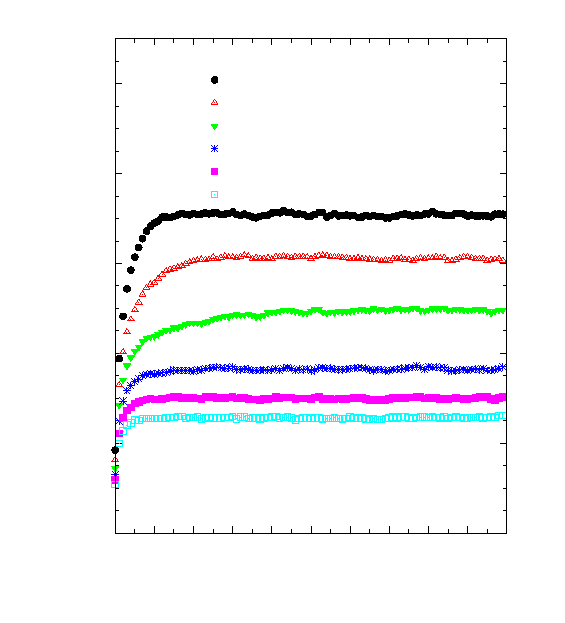
\includegraphics{comparisoncreutzreport}}%
    \gplfronttext
  \end{picture}%
\endgroup

%\end{figure} 

-average value of plaquette against number of steps for SU(2)->comparison to \citet{creutzsu2}, one picture

-autocorrelation, maybe one picture

-W(r,t) for different t, one picture

how to extract V(r) from W(r). fit values: maybe in appendix?

fit to potential, for one temperature each for SU(2) and SU(3)

\section{Discussion}

Differences between SU(2) and SU(3)? 
String tensions, also discuss differnet couplings/beta?->mnore figures, tables needed.

Areas for improvement: In Wilson-loops: also non-integer R, then also differnet orders of directions?
Link smearing
bigger lattices: a lot more computation time needed.

\section{Summary}

Reproduce confinement? Yes

%complicated way of specifying file, but does not need absolute path and simply writing refs did not work
\bibliography{../report/refs}

\end{document}

